\chapter{Das erste Kapitel}
\section{Using Abbreviations, Glossary and References}
\subsection{Abbreviations}
\subsubsection{Per Glossar}
Abbreviations short: \acrshort{DHBW}, \acrshort{I2CBus} 

and written out: \gls{DHBW}, \gls{I2CBus}

\subsubsection{Per acronym package}
Erste Erwähnung eines Akronyms wird ausgeschrieben mit Akürzung in Klammern angezeigt: \ac{AGPL}. Jede weitere wird nur in Kurzform verlinkt. Zweite Erwähnung: mehr zu \ac{AGPL} in \cite{fsf:2007}

\subsection{Citations etc}
References to Glossary:

 Singular: \gls{Glossareintrag}, Plural: \glspl{Glossareintrag}

Meine erste Fußnote\footnote{Ich bin eine Fußnote}

\subsubsection{BibTeX / Biber via blibliographie.bib}
Nur erwähnte Literaturverweise werden auch im Literaturverzeichnis gedruckt:
Indirektes Zitat (vgl. \cite{baumgartner:2002}) oder auch ein ``direktes Zitat'', \cite{dreyfus:1980}.

\textquote[{\cite[p. 35]{baumgartner:2002}}]{Direct citation which might span over several lines and thus should not be placed inline.}

%-----------------------------------------------------
% % possible alignments for wrapped figure:
% 
%    r, R - right side of the text.
%    l, L - left side of the text.
%    i, I - inside edge–near the binding (if [twoside] document).
%    o, O - outside edge–far from the binding.

\begin{wrapfigure}{R}{.4\textwidth}	% right aligned: r, allow to float (capital `R'/'L')
\includegraphics[height=.4\textwidth]{logo.png}
%\vspace{-15pt}	% push 15pt upwards
\caption{Das Logo der Musterfirma\footnotemark} % reference in footnote
\label{fig:logo-muster}
\end{wrapfigure}
\footnotetext{aus \cite{mustermann:2012}} % footnote text for above figure
%-----------------------------------------------------

\subsubsection{Reference via literatur.tex}
This doesn't work when biblatex is used:

\cite{bib:ix042010}, \cite{bib:metasploitBuch}
\paragraph{}
\textquote[{\cite[p. 35]{bib:metasploitBuch}}]{direct citation}.

\section{Figures}
Figure \ref{fig:logo-muster} shows a wrapped image.

Abbildung \ref{fig:ksmswing-diagramm} zeigt, dass ein kleines Bild zentral dargestellt werden kann...

\begin{figure}[ht!]
\centering
\includegraphics{images/logo.png}
%\includegraphics[width=\textwidth]{images/logo.png}
\caption{KSM/Swing Applikation \cite{mustermann:2012}}
\label{fig:ksmswing-diagramm}
\end{figure}


\section{lorem ipsum}
Looking for the one superhero comic you just have to read. Following the antics and adventures of May Mayday Parker, this Spider-book has everything you could want in a comic--action, laughs, mystery and someone in a Spidey suit. Collects Alias \#1-28, What If. Jessica Jones had Joined the Avengers. In her inaugural arc, Jessicas life immediately becomes expendable when she uncovers the potentially explosive secret of one heros true identity.

Once upon a time, Jessica Jones was a costumed super-hero, just not a very good one. First, a story where Wolverine and Hulk come together, and then Captain America and Cable meet up. In a city of Marvels, Jessica Jones never found her niche. The classic adventures of Spider-Man from the early days up until the 90s. Looking for the one superhero comic you just have to read.
